\chapter{ניהול סיכונים, תוכנית עבודה הנדסית, תקציב ומדדי הצלחה}
\label{ch:roadmap}

\section{ניהול סיכונים אסטרטגיים, טכנולוגיים וחוקתיים}
\label{sec:risks}
הטמעת תשתית לאומית להגנת התודעה כרוכה בסיכונים הדורשים מענה הנדסי ומוסדי מראש. טבלה~\ref{tab:risks} מסכמת את מפת שבעת הסיכונים המרכזיים ואת מערך הבלימה שתוכנן עבורם.

\begin{table}[htbp]
    \centering
    \caption{מטריצת ניהול סיכונים של פרויקט \textenglish{CivicShield AI} ודרכי מיטיגציה.}
    \label{tab:risks}
    \begin{tabular}{p{0.21\textwidth} p{0.10\textwidth} p{0.10\textwidth} p{0.37\textwidth} p{0.12\textwidth}}
        \hline
        \textbf{תיאור הסיכון} & \textbf{סבירות} & \textbf{חומרה} & \textbf{מנגנון בלימה ומיטיגציה הנדסית} & \textbf{סיכון שיורי} \\
        \hline
        התקפת \textenglish{Prompt Injection} בטקסט רשת & גבוהה & קריטית & אימות תחבירי קשיח (\textenglish{Pydantic JSON}), הפרדת הוראות מדאטה ובידוד סוכנים בארגז חול. & נמוך \\
        הטיה מפלגתית בסיווג מסגור & בינונית & קריטית & מבדק שוויון דו-מפלגתי שבועי (\textenglish{NFR-05}), פיקוח חוקתי וגילוי נאות בקוד פתוח. & נמוך \\
        התחמקות מתואמת (\textenglish{Adversarial Evasion}) & גבוהה & גבוהה & איחוד $4$ מודאליות בייסיאני (\textenglish{Audio/Video/C2PA/Graph}); התוקף נדרש לזייף את כולן יחד. & בינוני-נמוך \\
        צוואר בקבוק בזמן סגירת הקלפיות & בינונית & גבוהה & קנה מידה דינמי ל-$34\text{ GPU Pools}$ ושרידות \textenglish{Multi-AZ} תחת מודל \textenglish{M/M/c}. & נמוך \\
        דליפת מידע מזהה של אזרחים & נמוכה & קריטית & מחיקת \textenglish{PII} בכניסה, פרטיות דיפרנציאלית $\epsilon \le 1.2$ ומחיקה אוטומטית כל $30$ יום. & מזערי \\
        ניצול לרעה על ידי הרשות המבצעת & נמוכה & קריטית & מנגנון חתימה משולשת (\textenglish{3-of-3 Ed25519 Quorum}) כולל זכות וטו שיפוטית ואופוזיציונית. & מזערי \\
        עייפות תודעתית מאזהרות (\textenglish{Alert Fatigue}) & בינונית & בינונית & תזמון אזהרות ממוקד רק בחציית סף התפרצות $R_0 > 1.5$ והגבלת תדירות לציבור. & נמוך \\
        \hline
    \end{tabular}
\end{table}

\section{תוכנית עבודה הנדסית רב-שלבית ל-24 חודשים (Roadmap)}
\label{sec:roadmap}
הקמת מערכת \textenglish{CivicShield AI} מתוכננת בפריסה מדורגת על פני ארבעה שלבים בני חצי שנה כל אחד (סה''כ $24$ חודשים), כך שכבר בתום השנה הראשונה ניתן להפעיל תשתית צללים פאסיבית (\textenglish{Shadow Mode}) לצורכי כיול וביקורת טרם העלייה המבצעית המלאה:
\begin{itemize}
    \item \textbf{שלב א' (חודשים 1--6) --- תשתית קליטה, פרטיות ויומן ביקורת:} הקמת מאגרי \textenglish{Kafka/Flink} בארכיטקטורת \textenglish{Multi-AZ}, הטמעת מסנן $\epsilon$-\textenglish{DP}, בניית ארגזי החול ומערך הביקורת ה-\textenglish{Merkle}, וקליטת מדגם היסטורי לאימון ב-$3$ שפות.
    \item \textbf{שלב ב' (חודשים 7--12) --- ועדת הסוכנים ומנועי הפורנזיקה:} פיתוח ואימון של סוכני הרשת (\textenglish{CIB}), מסגור אנטמן בעברית ובערבית, גלאי ה-\textenglish{Deepfake} הבייסיאני ומנוע הסימולציות \textenglish{SIRI} ו-\textenglish{Hegselmann-Krause} ב-\textenglish{Python}.
    \item \textbf{שלב ג' (חודשים 13--18) --- שער חוקתי, משחקי מלחמה ואיזון פוליטי:} התקנת מנוע המדיניות \textenglish{OPA/Rego}, הטמעת מערכת החתימה הקריפטוגרפית המשולשת, וביצוע סדרת תרגילי צוות אדום (\textenglish{Red-Team Wargames}) עם אוניברסיטאות ומשפטנים.
    \item \textbf{שלב ד' (חודשים 19--24) --- הקשחה, אלסטיות והפעלה לאומית:} מבחני עומס של $12,000\text{ EPS}$ עם $34\text{ GPU Pools}$, חניכת פורטל השקיפות הפומבי וממשקי התקשורת, וקבלת תו כשירות סופי מוועדת הבחירות.
\end{itemize}

\begin{figure}[htbp]
    \centering
    % ============================================================================
% figures/fig_gantt.tex - Fig 7.1: 24-Month Engineering Roadmap Gantt Chart
% ============================================================================
\begin{tikzhebrew}[x=1cm, y=0.85cm]
  % Outer Frame
  \draw[csNavy, line width=1pt] (0, 0) rectangle (14.6, 6.2);

  % Top Navy Header Band
  \fill[csNavy] (0, 5.2) rectangle (14.6, 6.2);
  \node[white, font=\footnotesize\bfseries] at (2.5, 5.7) {\heb{שלב / תת-תוכנית הנדסית}};
  \node[white, font=\footnotesize\bfseries] at (9.8, 5.7) {\heb{לוח זמנים להקמה (חודשים 1 עד 24)}};

  % Timeline Header Row
  \fill[csNavyBg] (5.0, 4.55) rectangle (14.6, 5.2);
  \draw[csBorder] (5.0, 0) -- (5.0, 5.2);
  \foreach \x/\lbl in {5.5/M1, 7.65/M6, 9.8/M12, 11.95/M18, 14.1/M24} {
    \node[csNavy, font=\scriptsize\bfseries] at (\x, 4.88) {\lbl};
    \draw[csBorder, dashed] (\x, 0.85) -- (\x, 4.55);
  }

  % Row Labels (Right-aligned Hebrew inside left column)
  \node[anchor=east, font=\scriptsize\bfseries, csNavy] at (4.85, 3.95) {\heb{שלב א': תשתיות, \en{OSINT} ו-$\epsilon$-DP}};
  \node[anchor=east, font=\scriptsize\bfseries, csNavy] at (4.85, 3.05) {\heb{שלב ב': סוכנים, מסגור ו-\en{Deepfake}}};
  \node[anchor=east, font=\scriptsize\bfseries, csNavy] at (4.85, 2.15) {\heb{שלב ג': שער חוקתי ומשחקי \en{RedTeam}}};
  \node[anchor=east, font=\scriptsize\bfseries, csNavy] at (4.85, 1.25) {\heb{שלב ד': מבחני עומס \en{12k} והפעלה}};
  \node[anchor=east, font=\scriptsize\bfseries, csAmber] at (4.85, 0.42) {\heb{מבצעיות שוטפת ומבחני שוויון}};

  % Phase Bars
  \fill[csNavy, rounded corners=2pt]    (5.5, 3.72) rectangle (7.75, 4.18);
  \node[white, font=\tiny\bfseries] at (6.62, 3.95) {M1--M6};

  \fill[csNavy!75!csTeal, rounded corners=2pt] (7.45, 2.82) rectangle (10.2, 3.28);
  \node[white, font=\tiny\bfseries] at (8.82, 3.05) {M6--M13};

  \fill[csTeal, rounded corners=2pt]    (9.6, 1.92) rectangle (12.35, 2.38);
  \node[white, font=\tiny\bfseries] at (10.97, 2.15) {M12--M19};

  \fill[csTeal!75!green!65!black, rounded corners=2pt] (11.75, 1.02) rectangle (14.2, 1.48);
  \node[white, font=\tiny\bfseries] at (12.97, 1.25) {M18--M24};

  % Milestone Diamonds
  \foreach \mx/\my in {7.75/3.95, 10.2/3.05, 12.35/2.15, 14.2/1.25} {
    \node[diamond, fill=csCrimson, draw=white, line width=0.5pt, inner sep=1.8pt] at (\mx, \my) {};
  }

  % Continuous Audit Bar
  \fill[csAmber, rounded corners=2pt] (5.5, 0.2) rectangle (14.2, 0.64);
  \node[white, font=\tiny\bfseries] at (9.85, 0.42) {\heb{ביקורת שופטים ומבדק הטיה דו-שבועי}};
\end{tikzhebrew}

    \caption{מפת דרכים הנדסית ל-$24$ חודשים (\textenglish{Gantt}) להקמת והקשחת מערכת \textenglish{CivicShield AI}.}
    \label{fig:gantt}
\end{figure}

\section{תקציב חמש-שנתי, כלכלת טוקנים ותשואה מוסדית (ROI)}
\label{sec:budget}
בזכות תכנון הארכיטקטורה המדורגת (שכבה $2$ מפעילה סינון מהיר ומעבירה לשכבה $3$ רק $6\%$ לסוכן טריאז' ו-$0.8\%$ לוועדת ה-\textenglish{ReAct} המלאה), נחסכים כ-$94\%$ מעלויות ההסקה של מודלי השפה הגדולים, ועלות התפעול השוטפת נשמרת מאוזנת לאורך $5$ שנים. טבלה~\ref{tab:budget} ואיור~\ref{fig:roi} מפרטים את אומדן התקציב החמש-שנתי: עלות בעלות כוללת (\textenglish{Cumulative TCO}) של $68.7$ מיליון ש''ח מול ערך חוסן מוסדי מצטבר של $145.0$ מיליון ש''ח, עם נקודת איזון כלכלי (\textenglish{Break-Even}) בשנה $2.2$ (עודף נטו של $76.3$ מיליון ש''ח).

\begin{table}[htbp]
    \centering
    \caption{פירוט תקציב חמש-שנתי (\textenglish{CAPEX / OPEX}) וערך חוסן מוסדי (במיליוני ש''ח).}
    \label{tab:budget}
    \begin{tabular}{l c c c c p{0.34\textwidth}}
        \hline
        \textbf{שנת תוכנית} & \textbf{\textenglish{CAPEX}} & \textbf{\textenglish{OPEX}} & \textbf{סה''כ עלות} & \textbf{ערך חוסן} & \textbf{רכיב הוצאה מרכזי בתקציב} \\
        \hline
        שנה 1 (הקמה) & $14.5$ & $6.5$ & $21.0$ & $8.0$ & חומרת ליבה, צינור \textenglish{OSINT} ומודלי בסיס \\
        שנה 2 (שילוב) & $4.0$ & $8.2$ & $12.2$ & $22.0$ & רשת סוכנים, צוות אדום וכלי חיסון \\
        שנה 3 (בחירות) & $2.5$ & $8.8$ & $11.3$ & $31.0$ & שיא עומס אלסטי ($34\text{ Pools}$) ובלימת משברים \\
        שנה 4 (הרחבה) & $3.0$ & $9.4$ & $12.4$ & $38.0$ & תמיכה בבחירות מקומיות והנגשת \textenglish{XAI} \\
        שנה 5 (תחזוקה) & $2.0$ & $9.8$ & $11.8$ & $46.0$ & רענון מודלים אל מול טכנולוגיות זיוף עתידיות \\
        \hline
        \textbf{סה''כ 5 שנים} & \textbf{26.0} & \textbf{42.7} & \textbf{68.7} & \textbf{145.0} & \textbf{נקודת איזון (\textenglish{ROI Break-Even}) בשנה 2.2} \\
        \hline
    \end{tabular}
\end{table}

\begin{figure}[htbp]
    \centering
    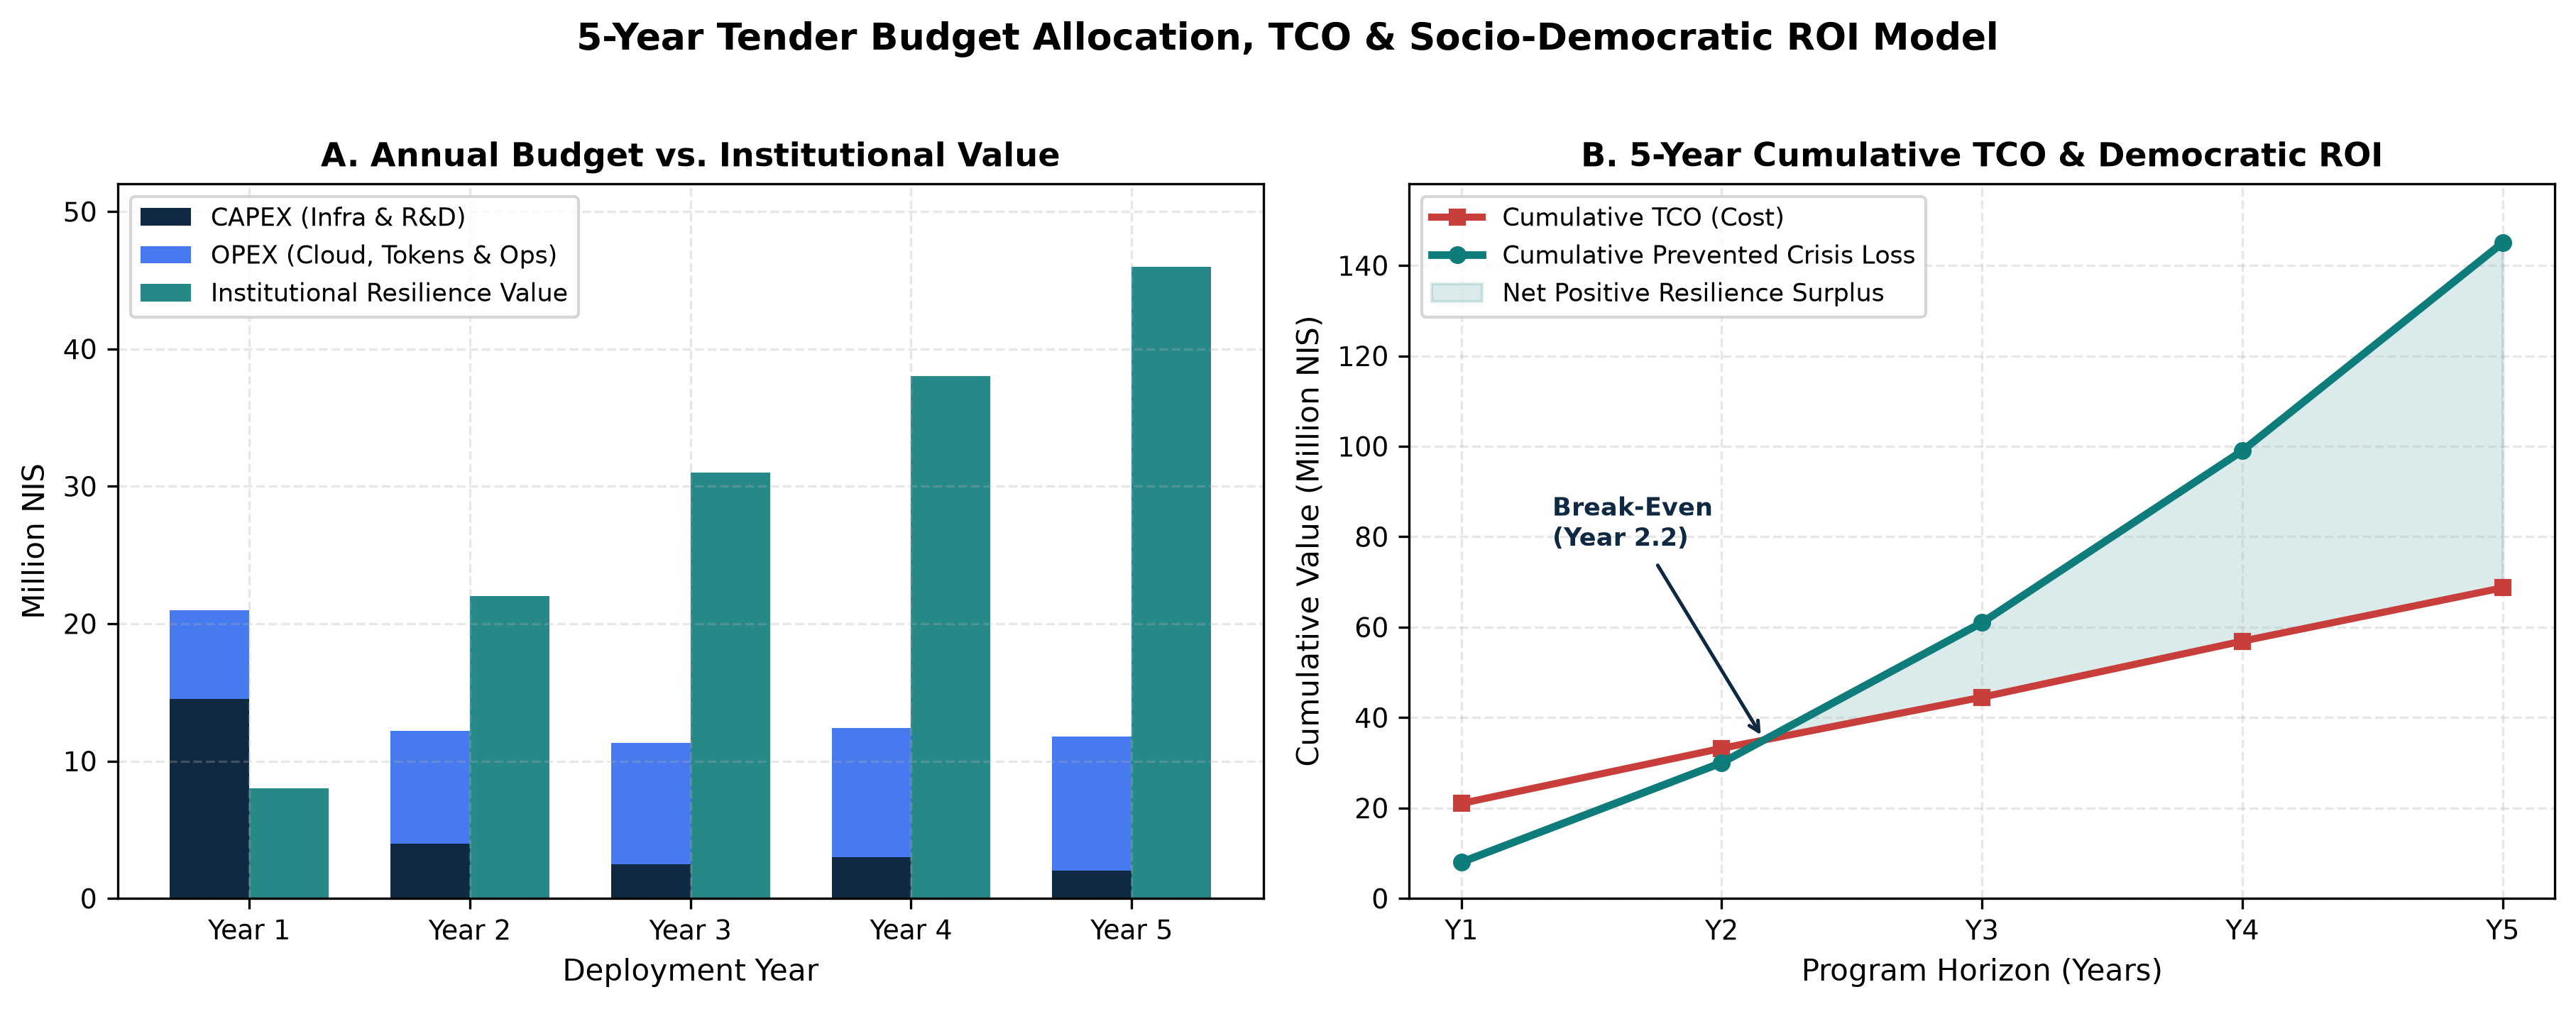
\includegraphics[width=0.96\textwidth]{figures/fig6_roi.png}
    \caption{תחזית תקציב חמש-שנתית (\textenglish{CAPEX/OPEX}), עלות בעלות כוללת (\textenglish{TCO}) והחזר השקעה מוסדי.}
    \label{fig:roi}
\end{figure}

\section{מדדי הצלחה מחייבים ורמת שירות (SLA / KPI Framework)}
\label{sec:kpi}
קבלת הפרויקט ומסירתו לידי ועדת הבחירות המרכזית ומערך הסייבר מותנות בעמידה מדידה בחמישה מדדי ליבה מרכזיים המפורטים בטבלה~\ref{tab:kpi}.

\begin{table}[htbp]
    \centering
    \caption{מסגרת מדדי הצלחה ורמות שירות (\textenglish{KPIs \& SLAs}) לתנאי מסירת הפרויקט.}
    \label{tab:kpi}
    \begin{tabular}{p{0.21\textwidth} p{0.18\textwidth} p{0.16\textwidth} p{0.35\textwidth}}
        \hline
        \textbf{שם המדד (\textenglish{KPI})} & \textbf{ערך סף מחייב} & \textbf{תדירות מדידה} & \textbf{שיטת אימות אובייקטיבית} \\
        \hline
        זמן תגובה בקצה (\textenglish{E2E Latency}) & $\le 250\text{ ms}$ & רציף (\textenglish{P95}) & מדידת שיהוי ב-\textenglish{Load Test} מול $12,000\text{ EPS}$. \\
        זמן גילוי והפקת \textenglish{Prebunking} & $\le 30$ דקות & לכל אירוע קריטי & חותמת זמן מרגע זריעה בטלגרם ועד הכנת תבנית חיסון. \\
        דיוק זיהוי \textenglish{Deepfake} משולב & $\text{Precision} \ge 90\%$ & חודשי + סקר תקופתי & ביקורת עיוורת על מאגר זיופים מבוקר בתיאום אקדמי. \\
        פער שוויון פוליטי (\textenglish{Fairness}) & $\Delta\text{FPR} < 1.5\%$ & דו-שבועי & הרצת סימולציית ביקורת סימטרית על כלל המחנות. \\
        אפס מקרי אכיפה ללא קוורום & $0$ חריגות & רציף (שער קריפטו) & אימות שלמות יומן ה-\textenglish{Merkle} ומפתחות ה-\textenglish{Ed25519}. \\
        \hline
    \end{tabular}
\end{table}
